\documentclass[11pt]{article}

\usepackage{amsmath}
\usepackage{amsfonts}
\usepackage{amssymb}

% Give ourself extra space for text
\usepackage[left = 2.2cm, right = 2.2cm, top = 1.8cm, bottom = 2.8cm]{geometry}

% Allows us to easily change the numbering system used in things like \begin{enumerate}. https://ctan.org/tex-archive/macros/latex/contrib/enumitem/
\usepackage[shortlabels]{enumitem}

% Turns table of contents, \refs, etc. into hyperlinks
\usepackage{hyperref}

% To include image, just use \includegraphics[scale=•]{relative path to image}
\usepackage{graphicx}
\graphicspath{ {./images/} }

% Common sets
\newcommand{\integers}{\mathbb{Z}}
\newcommand{\naturals}{\mathbb{N}}
\newcommand{\reals}{\mathbb{R}}

% Power set
\newcommand{\powerset}{\mathcal{P}}

% Identity matrix
\newcommand{\ident}{\mathbb{I}}

% Inverse hyperbolic functions
\DeclareMathOperator{\arcosh}{arcosh}
\DeclareMathOperator{\arsinh}{arsinh}
\DeclareMathOperator{\artanh}{artanh}

% I hat, J hat, K hat
\newcommand{\ihat}{\boldsymbol{\hat{\textbf{\i}}}}
\newcommand{\jhat}{\boldsymbol{\hat{\textbf{\j}}}}
\newcommand{\khat}{\boldsymbol{\hat{\textbf{k}}}}

% Better vectors (for single characters)
\renewcommand{\vec}[1]{\mathbf{#1}}

% Allows us to number equations in \begin{align} statements, etc.
\newcommand\numberthis{\addtocounter{equation}{1}\tag{\theequation}}

% Augmented matrices: this allows us to make augmented matrics using something like \begin{bmatrix}[cc|c]. Taken from Stefan Kottwitz at https://tex.stackexchange.com/questions/2233/whats-the-best-way-make-an-augmented-coefficient-matrix.
\makeatletter
\renewcommand*\env@matrix[1][*\c@MaxMatrixCols c]{%
  \hskip -\arraycolsep
  \let\@ifnextchar\new@ifnextchar
  \array{#1}}
\makeatother

% NOTE: This means \section does NOT number sections, but ensures that they appear in the table of contents, which does not occur if simply \section* is used. From egreg @ https://tex.stackexchange.com/a/30225.
\setcounter{secnumdepth}{0} % sections are level 1

\begin{document}
\title{ENG1005: Lecture 20}
\author{Lex Gallon}
\maketitle

\tableofcontents

\section*{Video link}
Click \href{https://echo360.org.au/lesson/G_32340f5d-ff38-43d2-be9d-d88ddb1b3611_b944cecf-8ba5-40d3-a870-0243a0a9e78c_2020-05-06T14:58:00.000_2020-05-06T15:53:00.000/classroom#sortDirection=desc}{here} for a recording of the lecture.

\section{Repeated eigenvalues §5.7.4}
If $A$ is an $n \times n$ matrix, then the characteristic polynomial of $A$ is 
\[ \text{c}(\lambda) = |A - \lambda \ident_n| = (\lambda - \lambda_1)^{m_1} (\lambda - \lambda_2)^{m_2} + ... + (\lambda - \lambda_p)^{m_p}\]

where
\begin{enumerate}[ (i) ]
\item the $\lambda_i$, $1 \leq i \leq p \leq n$, are the distinct roots ($\lambda_i \not = \lambda_j$ for $i \not = j$) of $\text{c}(\lambda)$ (in general, they are complex).
\item and the $m_i$, $1 \leq i \leq p$, is the algebraic multiplicity of the root $\lambda_i$.
\end{enumerate}

\subsection{Remarks}
\begin{enumerate}[ (a) ]
\item If $p < n$, then $A$ may not possess a complete set of eigenvectors.
\item If $m_i > 1$, then the number $n_i$ of linearly independent eigenvectors with associated eigenvalue $\lambda_i$ satisfies
\[ 1 \leq n_i \leq m_i \]
\end{enumerate}

\section{Parametric curves}
A parametric curve in $\reals^3$ (can do this in $\reals^n$ also) is a set of the form
\[ \mathcal{C} = \{ \vec{r}(t) | t \in (a, b) \} \quad (\text{ note whether interval is open or closed doesn't matter})\]
where
\[ \vec{r}(t) = (x(t), y(t)) \]

We call $\vec{r}(t)$ the \textbf{parametrisation} of the curve $\mathcal{C}$ (i.e. $\vec{r}(t)$ is NOT the curve). \\
The parametric curve $\mathcal{C}$ is said to be continuous (differentiable) if the parametrisation $\vec{r}(t)$ is continuous (differentiable). \\
If $\vec{r}(t)$ is differentiable, then we define
\[ \vec{r}'(t) = (x'(t), y'(t)) \]

\subsection{Examples}
\begin{enumerate}
\item $ \vec{r}(t) = (\cos(t), \sin(t)),\ 0 \leq t \leq 2\pi $. \\
Let $x = \cos(t),\ y = \sin(t)$, and then note that
\[ x^2 + y^2 = 1\]
So this parametrisation clearly traces out a circle.

\item $\vec{r}(t) = (t, t^2),\ t \in \reals$\\
Let $x=t$ and $y=t^2$ and then note that
\[ y = x^2 \]
So this parametrisation traces a parabola.
\end{enumerate}

\section{Tangent vectors}
\begin{center} 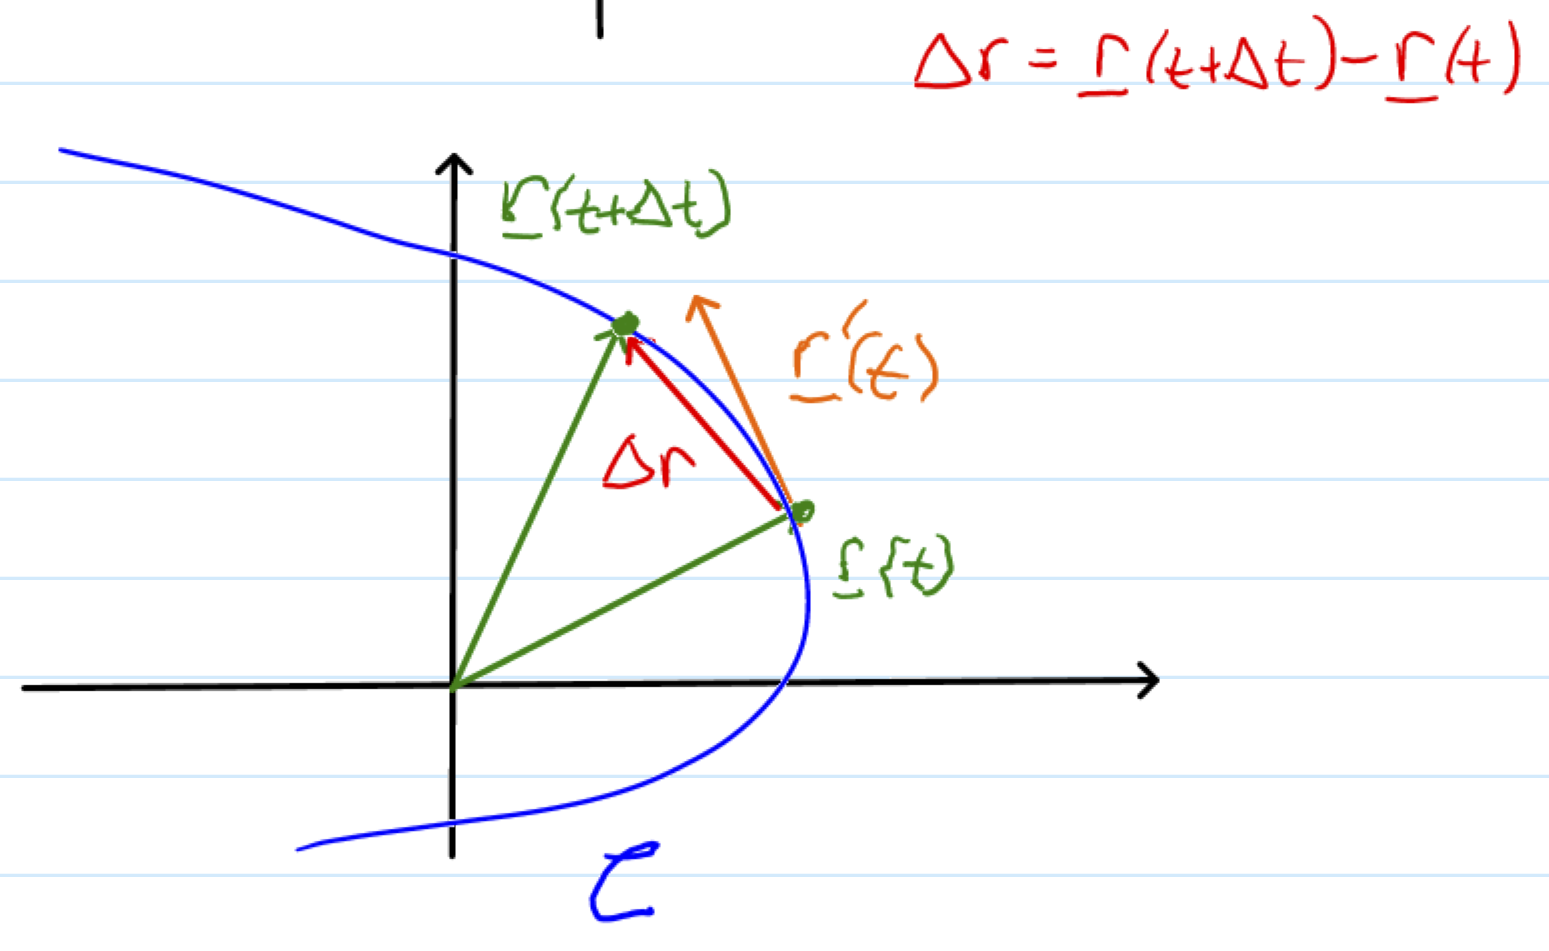
\includegraphics[scale=0.75]{tangent_vector} \end{center}

The approximate tangent vector is given by
\[ \frac{\Delta \vec{r}}{\Delta t} = \frac{\vec{r}(t + \Delta t) - \vec{r}(t)}{\Delta t} \]
So clearly, the tangent is given by
\[ \lim_{\Delta t \rightarrow 0} \frac{\vec{r}(t + \Delta t) - \vec{r}(t)}{\Delta t} = \vec{r}'(t) \]

So $\vec{r}'(t)$ gives a tangent vector to the parametric curve $\mathcal{C}$ at the point $\vec{r}(t)$.

\subsection{Example}
\[ \vec{r}(t) = (\cos(t), \sin(t)),\ 0 \leq t \leq 2\pi \]
Note: I already know that the tangent vector of a circle is at 90 degrees to the radius vector.

\[ \vec{r}'(t) = (-\sin(t), \cos(t)) \]
If this is indeed perpendicular to the radius vector then we would expect the dot product to be zero:
\begin{align*}
\Rightarrow \vec{r}(t) \cdot \vec{r}'(t) &= (\cos(t), \sin(t)) \cdot (-\sin(t), \cos(t)) \\
&= -\cos(t) \sin(t) + \sin(t) \cos(t) \\
&= 0
\end{align*} 

\section{Functions of several variables §9.6, 9.6.1}
\subsection{Definition}
A function of $n$ variables, denoted $f(\vec{x}),\ (\vec{x} = (x_1, x_2, ..., x_n))$ is a rule that associates to each point $\vec{x} \in D \subset \reals^n$, $D$ is called the domain, a number $f(\vec{x}) \in \reals$; symbolically, we write
\[ f: D \subset \reals^n \rightarrow \reals : \vec{x} \mapsto f(\vec{x}) \]
Note that $f(\vec{x})$ is \textit{usually} defined by a formula.

\subsection{Examples}
\begin{enumerate}[ (a) ]
\item $f(x, y) = \ln(x^2 + y^2)$. We can assume $D = \reals^2 \backslash \{(0, 0) \}$
\item $f(x, y, z) = e^{xyz},\ D = \reals^3$
\end{enumerate}

\section{Parametric surfaces}
\subsection{Definition}
A parametric surface inf $\reals^3$ is a set $S$ that is defined by
\[ S = \{ \vec{r}(u,v) \} | (u, v) \subset D \subset \reals^2 \]
where $\vec{r}(u, v) = (x(u,v), y(u, v), z(u, v))$.\\
We call $\vec{r}(u, v)$ the \textbf{parametrisation} (or parametric equation) of $S$.

An important special case of a parametric surface is the graph of a function $f(x, y)$ that is defined by
\[ S = \{ (x,y, f(x,y)) | (x, y) \in D \} \]
\begin{center} 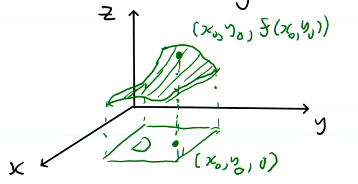
\includegraphics[scale=1.5]{parametric_surface} \end{center}

\end{document}